

\chapter{Introduction}
\label{chap:introduction}
\setcounter{page}{1}
\pagenumbering{arabic}
Consumer applications have existed on the web for more than a decade now. Amongst others, e-mail, time management, social collaboration and file sharing applications can all be accessed using a web browser. For consumers, the main advantages are the independence of special software and the ability to access their data from nearly any computer, but web applications are also an interesting approach for enterprise solutions: In opposition to desktop applications, web applications do not need to be installed on end-user machines. This advantage is complemented by the fact that the roll-out of updates can easily be performed on the server-side only.

Until recently, browsers were not powerful enough for desktop-level, complex end-user clients. But as rendering techniques and JavaScript engines get faster, the possibilities of \glspl{bba} grow. In combination with JavaScript frameworks, web browsers become a runtime environment, powerful enough to build applications that can replace traditional end-user clients.

The \acl{mvc} pattern is a commonly used architectural design pattern. Being based on the principle of \emph{Separation of Concerns}, it helps to structure an application by dividing it into three different parts: the Model, which holds business data, the View, which displays these data, and the Controller, which is responsible for user interaction.

MVC was created in the 1970s, long before the world wide web became popular, and has been used in many desktop applications since. But applying it to the domain of web applications introduces a challenge: the web is a distributed computing environment. While it is rather simple to connect MVC components inside a monolithic desktop application, distributing them across different tiers --- at least \emph{client} and \emph{server} --- opens up possibilities for different implementations. With respect to three defined criteria, this thesis investigates and evaluates different web application architectures based on the Model-View-Controller pattern.

\glsunset{ibm}
\glsunset{cn}
\section{Motivation and Scope}
In the following section, \emph{IBM Content Navigator}, one of IBM's most recent web clients, is introduced. By connecting it to \acl{ecm} and SmartCloud Content Management, the business problem that leads to the goals of this thesis is explained.

%\subsection*{Web Applications within IBM}
%The \ac{ibm} corporation has recognized the advantages that browser-based applications have for enterprise solutions. Several products of IBM are or are accompanied by web clients, such as \emph{Connections}\footnote{See \url{http://www-01.ibm.com/software/lotus/products/connections/}}, a social software for companies, or \emph{LotusLive}\footnote{See \url{https://www.ibm.com/cloud-computing/social/us/en/webmeetings/}}, a web meeting tool. IBM also builds software to create web applications, for example the IBM Web Experience Factory\footnote{See \url{http://www-01.ibm.com/software/genservers/webexperiencefactory/}}.

% Part of the company's long term strategy regarding web applications is \emph{The Dojo Toolkit}. Dojo is an open source JavaScript framework to build rich, client-side web experiences based on widgets and the \emph{AJAX} technique. It is used throughout IBM's web application portfolio. Recently\footnote{See \url{http://maqetta.org/index.php?view=article&catid=2&Itemid=9&id=28}}, IBM contributed \emph{Maqetta} as open source to the Dojo Foundation\footnote{The foundation is backing the development of Dojo.}. Maqetta is a visual authoring tool for creating HTML5 web applications based on Dojo.

%IBM provides guidelines to unify the User Experience\footnote{The look and feel of a \ac{ui}.} of web applications, known as \emph{OneUI}. There are also IBM internal extensions to Dojo that primarily enhance existing \glspl{widget}, called the \emph{\ac{idx}}.

\subsection*{Enterprise Content Management and IBM Content Navigator}
According to \citeasnoun{wiki:ecm}, ``\ac{ecm} is a formalized means of organizing and storing an organization's documents, and other content, that relate to the organization's processes. The term encompasses strategies, methods, and tools used throughout the lifecycle of the content.'' Contracts, invoices, orders or insurance policies are all examples for such content. IBM offers different solutions for \ac{ecm}, three of them being \glspl{repository} to manage digital documents: \emph{\gls{p8} (P8)}, \emph{\gls{cm} (CM)} and \emph{ContentManager OnDemand (OD)}. All three are complemented by web clients used to access the repositories (e.g. to upload, download, or move documents): \emph{Workplace XT} for FileNet and \emph{WEBi} for CM and OD. They are usually delivered with every solution that also includes their respective repository software.

%\ac{ibm} adresses \ac{ecm} with two solutions to manage digital documents: \emph{\gls{p8}} and \emph{\gls{cm}}. Both are complemented by web clients used to access the repositories (e.g. to upload, download, or move documents): \emph{Workplace XT} for FileNet and \emph{WEBi} for ContentManager.

Amongst other clients of IBM ECM products, Workplace XT and WEBi are going to be replaced by \ac{icn}\footnote{See \url{http://www-01.ibm.com/software/ecm/experience.html}}. This new web application allows access to FileNet, ContentManager and ContentManager OnDemand repositories through a single \acl{ui}. 
IBM Content Navigator is a Rich Client based on the \acl{mvc} pattern. It makes use of \emph{The Dojo Toolkit}, which is an open source JavaScript framework to build rich, client-side web experiences based on widgets and the \emph{AJAX} technique. Dojo is the standard framework used by most of the IBM web clients.
ICN follows IBM OneUI, which is an initiative within IBM to unify the user experience\footnote{The look and feel of a \acl{ui}.} in products' web clients by providing guidelines. Content Navigator also makes use of IBM internal extensions to Dojo, called the \emph{\acl{idx}}, which primarily enhance existing Dojo widgets to follow the OneUI standards.

%Built on the \acs{ajax} technique and \emph{The Dojo Toolkit}, and following the OneUI guidelines, Content Navigator is a Rich Client following the MVC pattern.

\begin{figure}[H]
	\centering
	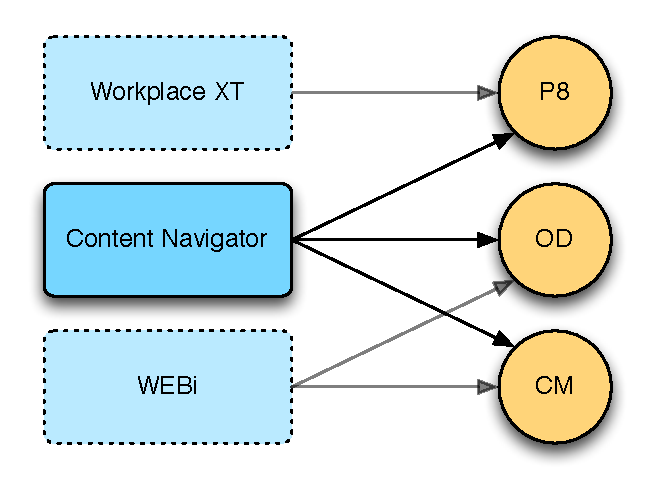
\includegraphics[width=10cm]{images/nexus.pdf}
	\caption{IBM Content Navigator replaces WEBi and Workplace XT}
	\label{fig:nexusp8cmod}
\end{figure}

Due to its plug-in based architecture, IBM Content Navigator can not only be used as a distinct application, but also as a framework which can be used to build arbitrary web applications. Although originally built with the access to ECM content repositories as a core feature, web applications developed on top of \ac{icn} can serve any purpose.

\nexus\ makes integration of different applications possible through two features:
\begin{itemize}
	\item A plug--in system that allows developers to create extensions for every purpose and on every layer with both server-side and client-side features
	\item A client-oriented \ac{mvc} architecture that provides the structure for the rich, browser-based application
\end{itemize}

\subsection*{SmartCloud Content Management}
IBM \ac{sccm} is a \ac{saas} offering for document and email compliance archiving. It is part of IBM's ECM portfolio and integrates different IBM products to deliver an out-of-the-box archiving solution for enterprises. One of these integrated products is the document management system \emph{FileNet P8} and its web client, \emph{Workplace XT}. In addition to Workplace XT, SCCM also provides a browser-based administration interface.

As Workplace XT is going to be replaced by \ac{icn}, it is planned to port the SCCM administration interface to the \ac{icn} platform for the next release, too. This integration will provide customers with a unified \acl{ui} for the different web clients delivered through SCCM.

\subsection*{Goals and Scope}
As a first goal, this thesis demonstrates how the \ac{mvc} pattern can best be implemented in web applications. Based on three defined criteria, different MVC-based web application architectures are evaluated to investigate the shift to rich, JavaScript-based clients.

The second goal of this thesis is to investigate and present the part of the IBM Content Navigator architecture related to the MVC pattern. In conjunction with the thesis of Robert Metzger, a working prototype of an ICN plug-in was developed to approach a problem being faced with the SCCM cloud offering. The plug-in demonstrates how the MVC pattern can be implemented in practice and should help the SCCM development team to get up to speed with porting the SCCM administration interface to IBM Content Navigator.

It is not in the scope of this thesis to create a new way to implement MVC in web applications. It is also neither a goal to find and list all possible implementations of MVC architecture on the web, nor to find the single best way to implement it. Instead, four MVC architectures and their applicability are compared to identify the one that best fulfills an application's requirements.
\newpage
\section{Document Structure}
\emph{Chapter One, ``\nameref{chap:introduction}''} explains the motivation behind this thesis. It familiarizes the reader with the business background, defines goals and outlines the document structure.

\emph{Chapter Two, ``\nameref{chap:mvc}''} introduces \acs{mvc}, its history and origins in \mbox{Smalltalk-80}, its structure and the tasks of the different components. It also presents two variations of \ac{mvc} --- MVP and MVVM --- which are commonly used in web applications.

\emph{Chapter Three, ``\nameref{chap:webapparch}''} describes technologies and techniques relevant to web application architecture and explains the terms \emph{Thin Client} and \emph{Rich Client}.

\emph{Chapter Four, ``\nameref{chap:webmvc}''} gives examples of problems that emerge with web applications and defines these problems as criteria. After that, various possibilities to implement \ac{mvc} in client--server architectures are discussed based on the previously defined criteria.

\emph{Chapter Five, ``\nameref{chap:nexus}''} presents \acl{icn} and examines its plug--in system and architecture. Hereafter, the design of a log analysis plug--in developed in the course of this thesis is discussed further.

\emph{Chapter Six, ``\nameref{chap:conclusion}''} summarizes the findings and gives an outlook on web application architecture with respect to current developments and evolving standards.